\paragraph\
  Flow monitoring protocols like NetFlow\cite{NetFlow} and sFlow\cite{sFlow} can provide important information about traffic that passes
  through a network. However contemporary computer networking is out-spacing out ability to monitor them efficiently.
  As data centers are getting virtualized with virtual software switches and scaling to thousands of node, it is our 
  immediate requirement to have monitoring system  that can scale efficiently. There are few solutions that provide 
  some methods to have scalable flow monitoring in data center networks.
  
  \section{EMC2\cite{emc2}} %expasion of EMC2 
  \paragraph\
  EMC2 is a scalable network wide monitoring service for data centers. EMC2 stays inside host computer  to monitor virtual switches.
  Monitoring at virtual switch is scalable due to its distributed nature.
  
  \subsection{Architecture}% what exacly happen not only level arcs in image  % modul
  \paragraph\
    EMC2 is a multi-threaded application that spawns parser thread upon accepting sFlow/NetFlow packets. EMC2 maintains 
    a 2-level in-memory hash table that contains flow records. Layer-3 source and destination address forms Flow-ID that acts as 
    primary key for in-memory hash table. Flow-ID maps to another hash table where timestamp is the key and flow record is value. 
    Flow record contains number of packets, number of bytes and optional path vector.
    \begin{figure}[h!]
      \centering
          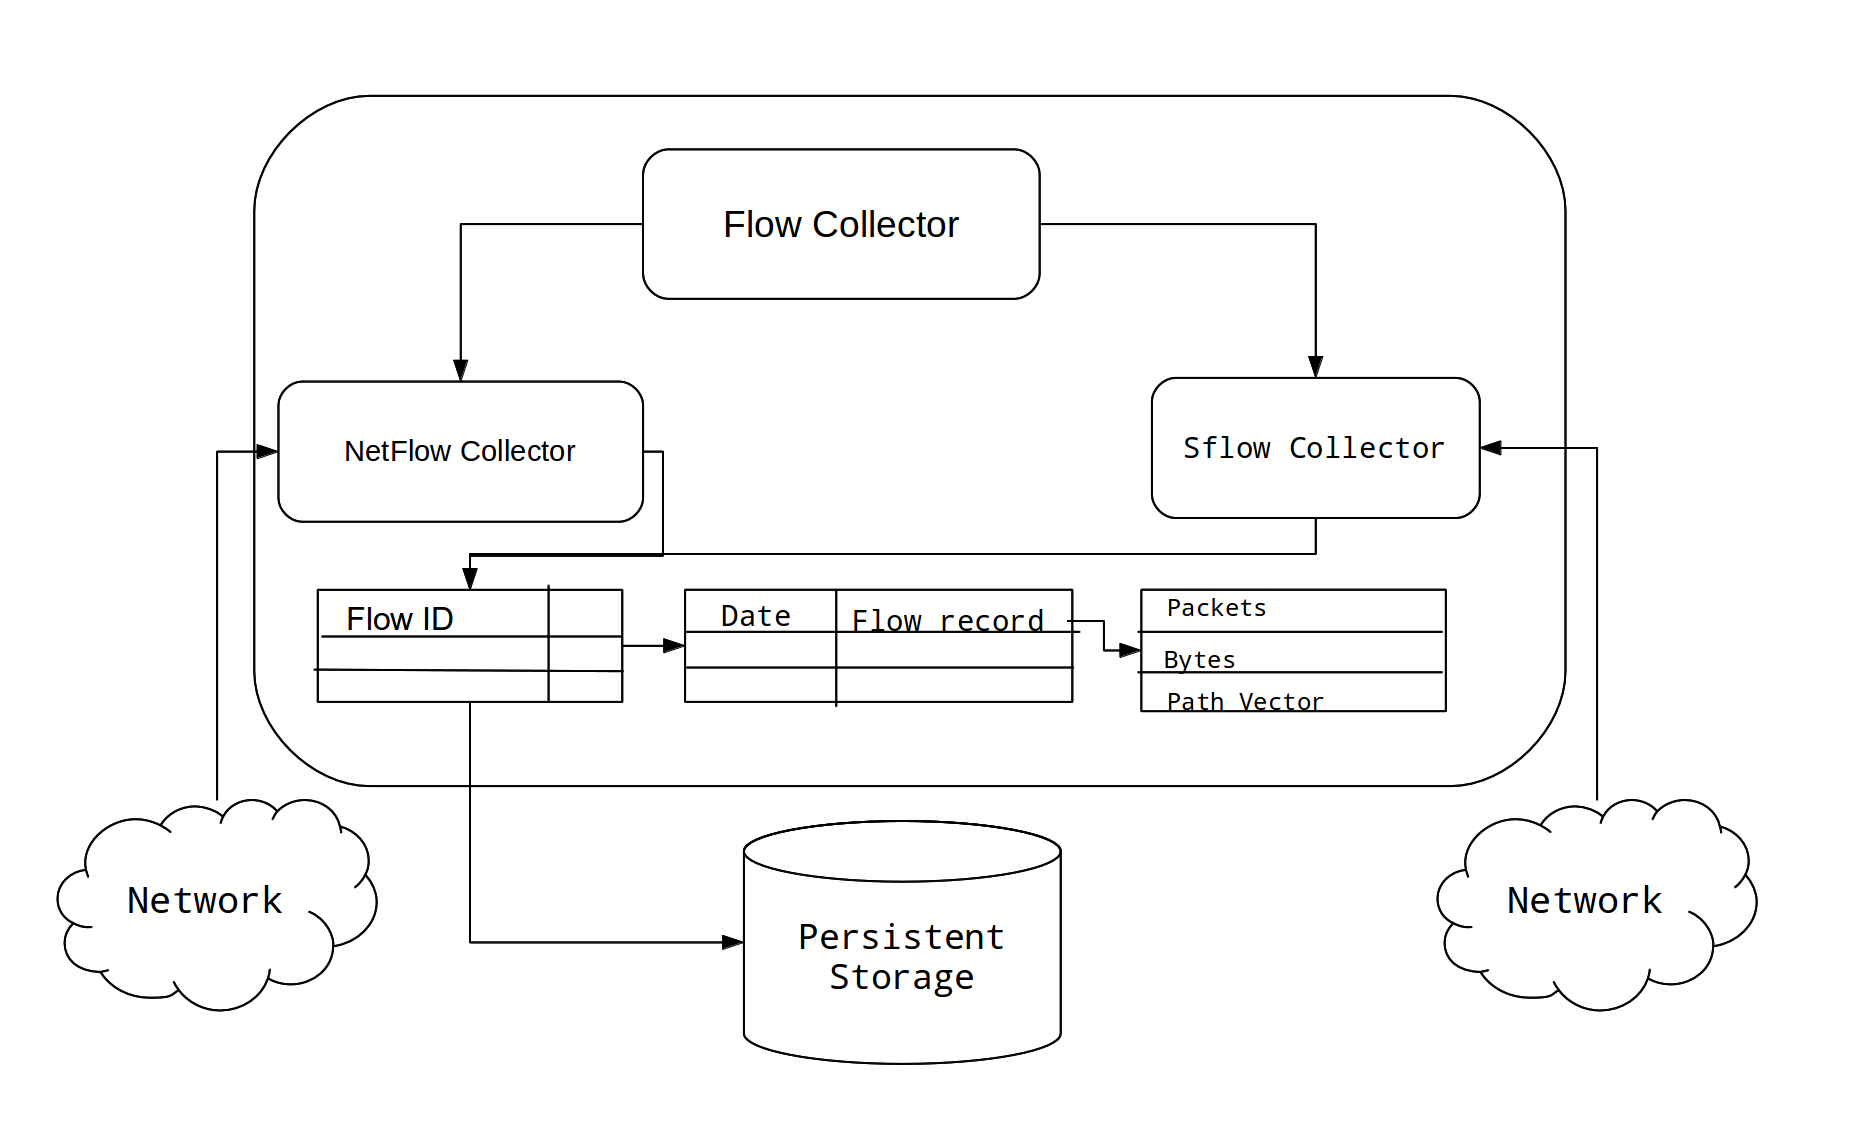
\includegraphics[scale=.3]{emc2.png}
          \caption{Architecture of EMC2.} % Give ref % label arcs % draw by urself
    \end{figure}
    
    \subsection{Deduplication}
      \paragraph\
      Deduplication avoids adding of same flow in the flow table reported by multiple Vswitchs for the same flow.      
      EMC2 uses simple heuristics to to detect duplicate flow.\\

     
      \begin{algorithm}[H]
        \caption{Detect Duplicate Flow}
	\label{alg1}
	\begin{algorithmic}
	  \IF{$flow-ID$ not exist}
	      \STATE add flow to the flow table.
	      \RETURN 
	  \ELSE 
	      \IF {Same exporter}
		  \STATE update the flow table.
		  \RETURN 
	      \ELSE
	        \STATE report duplicate flow.
	        \STATE update path vector.
	        \RETURN 
	      \ENDIF
	  \ENDIF
	\end{algorithmic}
       \end{algorithm}
      \pagebreak
    \subsection{Data Rate Prediction in Presence of Sampling}
    \paragraph\
    EMC2  predict data rate my multiplying length of the packet with sampling rate given in flow packet.
    It can also report low sampling rate by accumulating samples from different exported devices. 
    \subsection{Advantages and Limitations}
    Advantages of EMC2 are
    \begin{itemize}
     \item Scalable and distributed monitoring.% no distrubuted % claimed advantages of emc2% why they claim scalable
     \item %scalabe arise distribuyed storage 
     %monitorng of network will be diffucult .
     \item In-memory flow table for fast flow update.% everybody does that.
    \end{itemize}
    Disadvantages are
    
     \begin{itemize}
      \item Lack of scalable storage.
      \item Centralized monitoring will be difficult as it needs to fetch from distributed flats files.
     \end{itemize}

  \section{TS}